\hypertarget{RelatedWork}{
%\label{Textons}\index{Textons@{Texton Dictionary}}}
}
In earlier research on the topic of material recognition, a lot of focus was on the albedo variation on top of a flat surface. More recently, this focus has shifted towards surface normals, which cause the 3D effects we perceive. In this section, some state-of-the-art methods are outlined.

\section{Textons}\label{sec:Textons}

The need for larger texture databases that captures the variety in viewpoint and illumination resulted in the creation of the CUReT database \cite{DanaNayar}. Dana and Nayar developed parametric models based on surface roughness and correlation lenghts which were tested against the CUReT database. However, in their research, no significant results were reported \cite{VarmaZisserman}.

Leung and Malik were the first to introduce the texton modeling method to the problem of illumination variation \cite{LeungMalik}. In their research, they introduce the concept of 2 and 3-dimensional textons based on Gaussian derivative filters. The idea is that these Gaussian filters capture certain properties of a texture on microscale; for example, a point $n(x,y)$ in an image of a texture can correspond to a ridge, bump, groove, spot, etc. A filter-bank of different Gaussian filters can capture these properties in the response of the image applied to such filter. This makes it able to capture the variance of textures under different illuminations using a representable set of filteres.

\begin{figure}[b]
	\begin{center}
		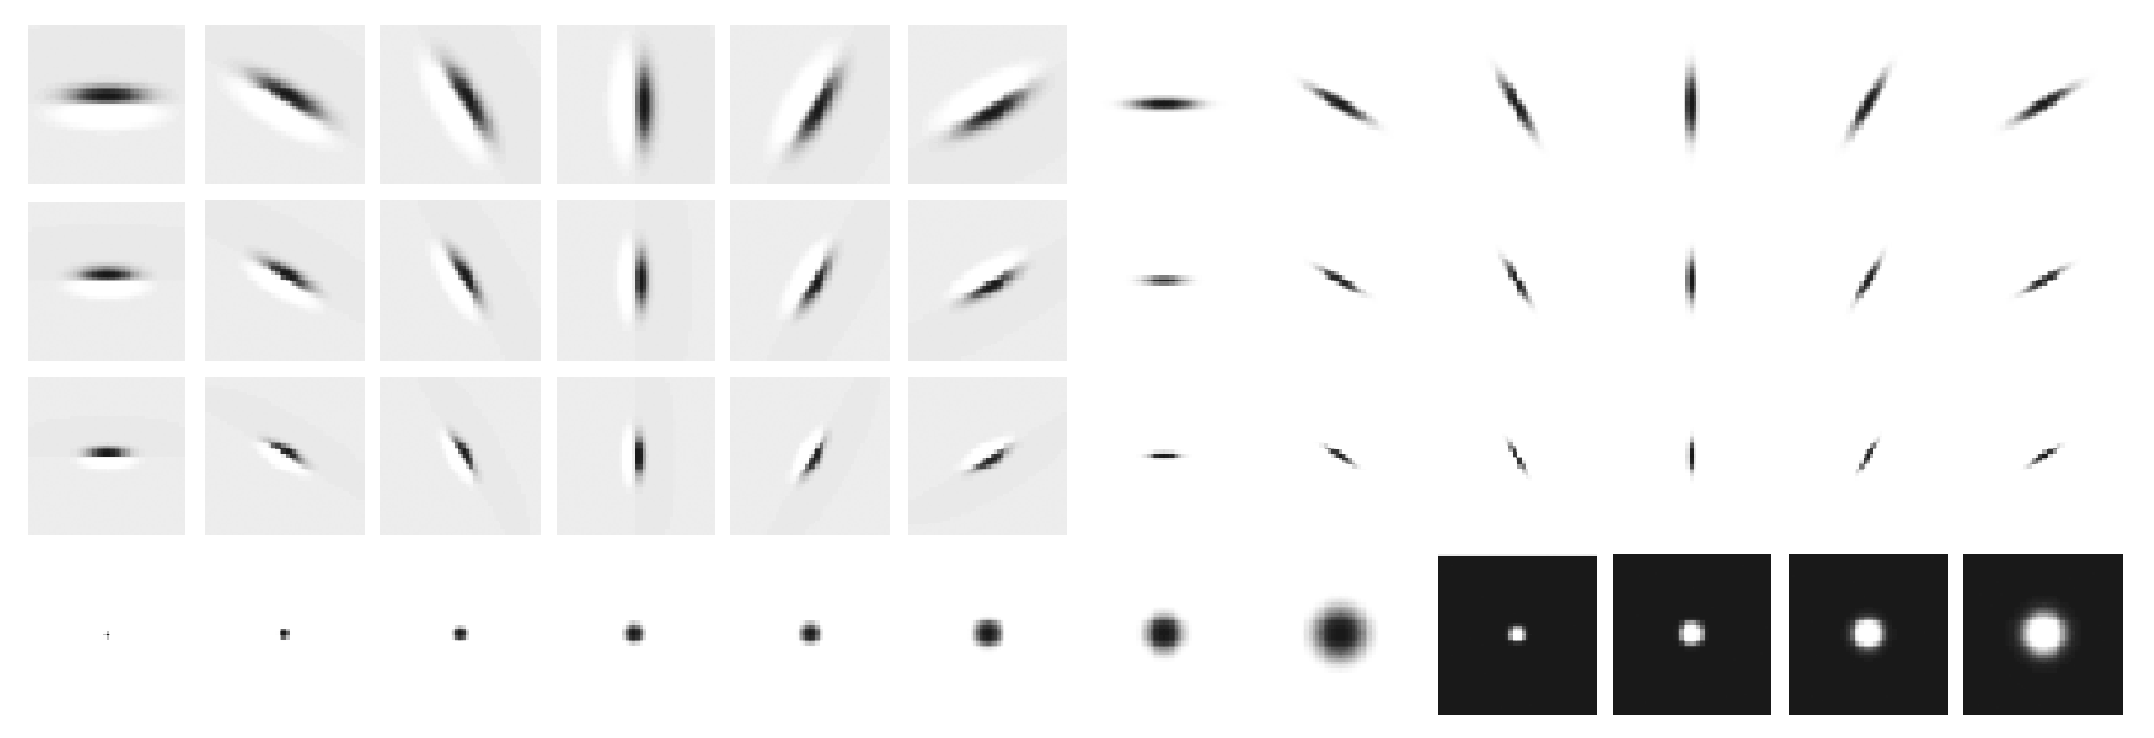
\epsfig{file=images/LM.eps, width=0.6\linewidth}
	\end{center}
	\caption{\textit{LM filter bank, consisting of an edge, bar and spot filter at multiple orientations and scales. 2 Gaussian derivatives at 6 orientations and 3 scales, 8 Laplacian of Gaussian filters and 4 Gaussian filters give a total of 48 filters in the filter bank.}}
	\label{fig:LM}
\end{figure}


In the case of a 2D texton, a texture is being characterized by responses obtained by convolving images from this texture with a set of orientation- and spatial-frequency linear filters. As a result, every pixel in an image is now represented as a vector of $N_{fil}$ corresponding response values, where $N_{fil}$ is the number of filters in the filter bank. With the obtained set of vectors size $N_{fil}$, they use a K-means algorithm to find a number of vectors as representable clusters in this vector space. The clusters found by K-means this way are the 2D textons descriptors. These textons represent characteristics such as ridges, bumps, etc. of the texture under a given illumination.

Because a texture under a different illumination can appear completely changed due to effects of masking, shadowing, specularity or global illumination, a 2D texton is not enough to capture the general characteristics of a texture. A good example of how textures change under illumination is shown in figure X. A great deal of shadows and masking effects make it hard to classify image $b$ when the textons are computed from image $a$, since these effects are not properly quantized to the textons. 

To capture such effects, many images with different illumination variation and viewing directions are needed. Given a number of images $N_{img} >> 1$,  concatenating the responses of these $N_{img}$ images will give long $N_{fil}N_{img}$ data vectors. Clustering these data vectors with K-means will give cluster centers which encode the dominant properties in all the images belonging to a certain texture class. These cluster centers represent the 3D textons and encode various image properties like illumination changes, spatial properties (bumps, ridges, etc.), as well as reflectance properties of the material (shiny/glossy as well as diffuse properties). Given the wide range of features 3D textons can capture make them strong descriptors for the problem of illumination variation within texture classification.

The set of 3D textons (K-means cluster centers) over all classes will serve as a Texton Dictionary for the construction of histograms. Using the same responses as before, for a training image, a histogram is constructed by assigning every vector corresponding to a pixel in the image to a texton in the dictionary using the $\chi^2$ (Chi Square) statistic to measure distance between vector and textons. The histogram is a representation of the image in terms of features, as encoded in the texton dictionary. With this quantization procedure, each texture-class can be represented by a set of histograms. To classify a novel image, responses are computed, a histogram is constructed from the texton dictionary, and a Nearest Neighbor algorithm is applied to find a histogram in the training set closest to it. The function to measure distances between histograms is again $\chi^2$.

Originally, Leung and Malik used a set of 48 Gaussian derivative filters to compute the responses on an image. Varma and Zisserman extended this research by observing the effect of various filter banks for the computation of the responses \cite{VarmaZisserman}. In their experiments, with a similar setup, they constructed texton dictionaries based on different filter banks and compared them to the filter bank proposed by Leung and Malik. The filter banks used in these experiments were the Schmid (S) set and the Maximum Response (MR) sets. 

The S set consists of 13 isotropic Gabor-like filters rotationally invariant filters.

The MR sets consist of 38 Gaussian derivative filters: 2 anisotropic filters for edges and bars, on 6 orientations and 3 scales, and 2 isotropic filters, a Gaussian and a Laplacian of a Gaussian filter. They used two version of this set in their experiments. The MR8 set, only the top 8 responses are recorded by taking the maximum response of the anisotropic at each scale over all orientations and taking the responses of both isotropic filters. The MR4 set is a subset of the MR8 set, where the anisotropic filters only occur on a single fixed orientation.

The experiments showed a significant difference in performance for the different filter banks, with the MR8 filter bank giving the best classification accuracy. 

\begin{figure}[t]
	\begin{center}
		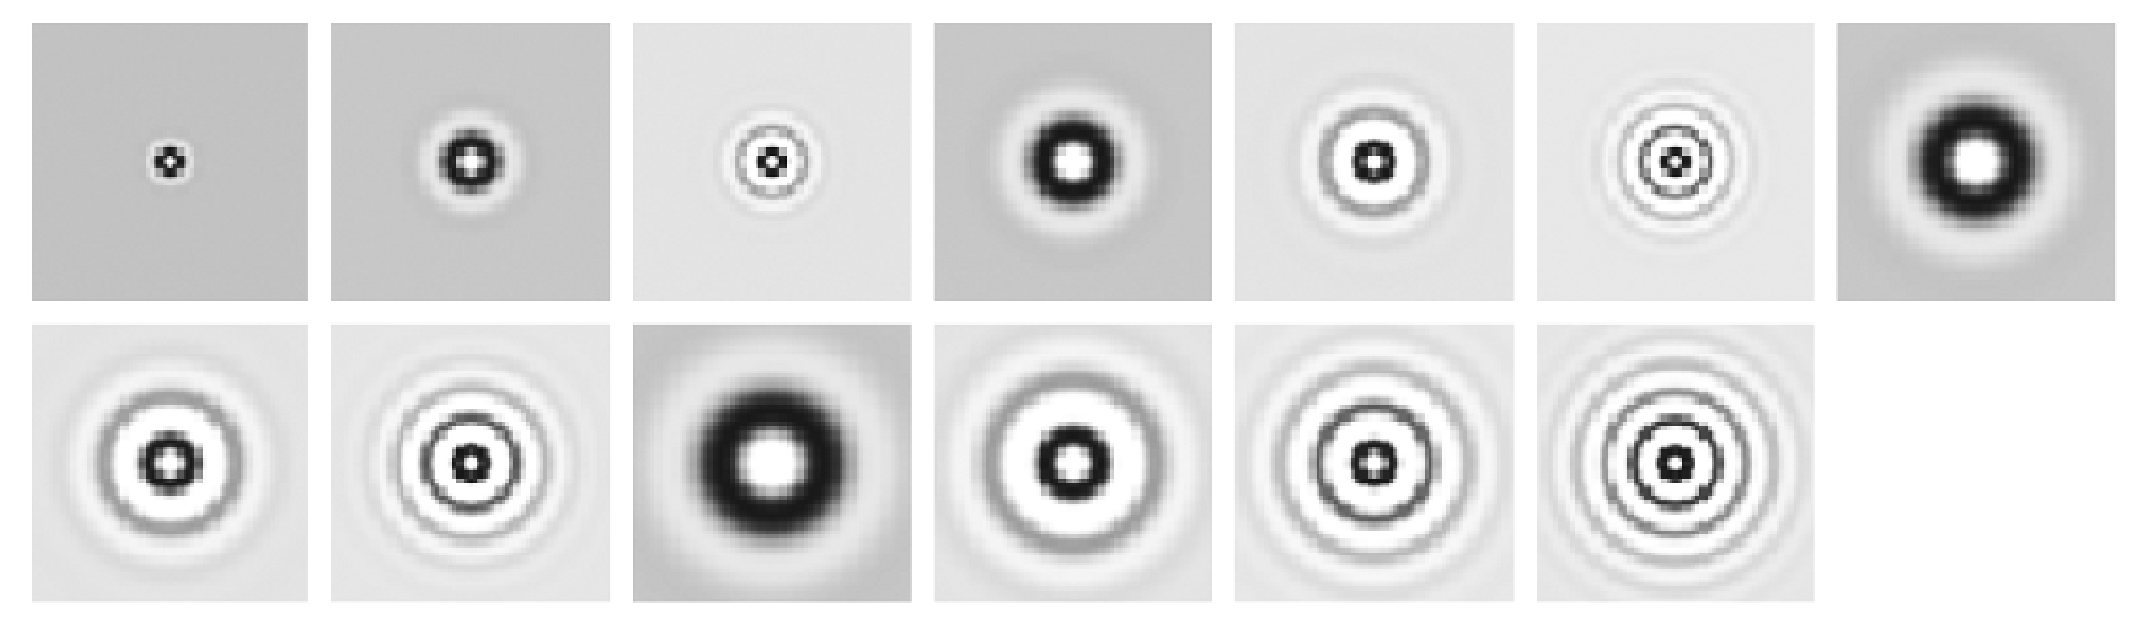
\epsfig{file=images/S.eps, width=0.6\linewidth}
	\end{center}
	\caption{\textit{The Schmid filter bank consists of 13 isotropic rotationally invariant filters.}}
	\label{fig:S}
\end{figure}

\begin{figure}[b]
	\begin{center}
		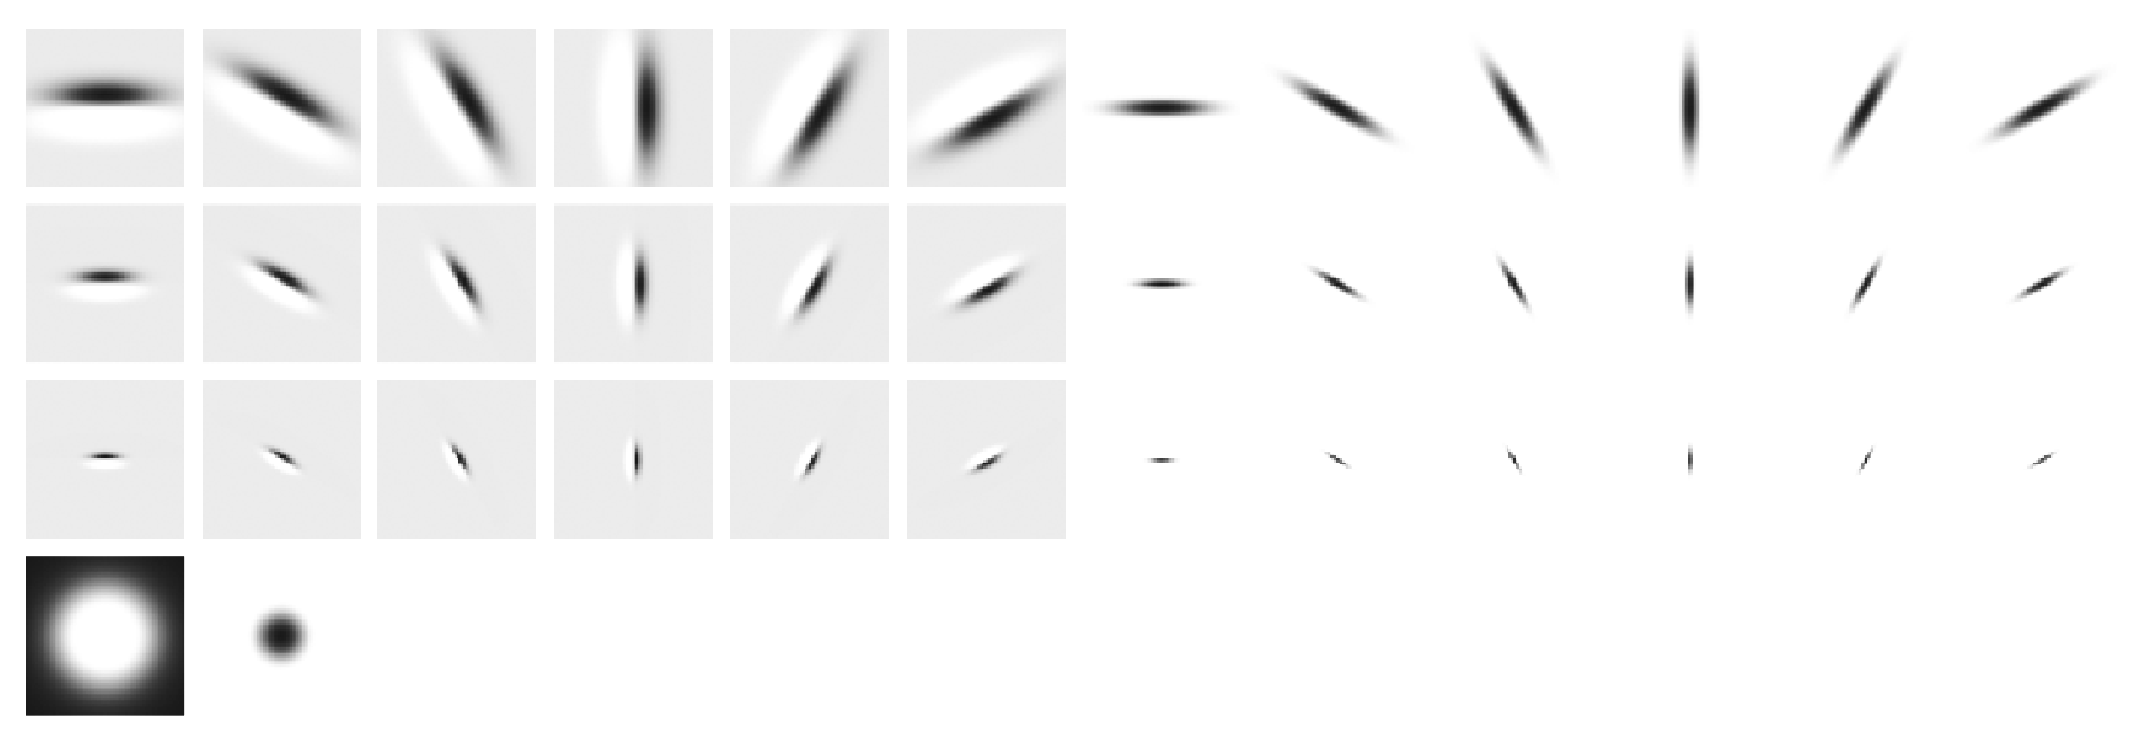
\epsfig{file=images/MR.eps, width=0.6\linewidth}
	\end{center}
	\caption{\textit{The Maximum Response filter bank consisting of 2 anisotropic edge and bar filters at 6 orientations and 3 scales and 2 isotropic filters, a Gaussian and Laplacian of Gaussian. A total of 38 filters, but only 6 filter responses of the anisotropic filters across orientations and the 2 responses of the isotropic filters are registered.}}
	\label{fig:MR}
\end{figure}

\section{Multivariate Gaussian Distributions}\label{sec:MGD}
A drawback of the texton approach is the need for a construction of the texton dictionary, because it needs clustering in high-dimensional spaces. This poses problems when the number of classes and image data increase as it becomes intractable to compute the clusters, but at the same time, the idea of using textons implicates that more data is needed to capture general properties correctly.

Broadhurst presents a parametric approach to estimate the likelihood of homogeneously textured images \cite{Broadhurst}. His work extends the framework proposed by Levina \cite{Levina} by using a Gaussian Bayes classifier instead of a Nearest Neighbor classifier. To model each texture class, Broadhurst uses multivariate Gaussian distributions to model the intra-class variability of each marginal histogram. This is done by mapping the joint marginal histograms into Euclidean space and applying PCA to obtain eigencomponents for each class.

Marginal distributions of each filter response are estimated by using non-parametric histograms. There are several advantages to this:

\begin{enumerate}
	\item This approach eliminates effectively the need of a texton dictionary. The use of a dictionary limits the generalization of a texture class and also needs clustering in high-dimensional spaces, making the problem intractable when extending the number of classes.
	\item Marginal distributions can be estimated accurately, while joint distributions often suffer from the curse of dimensionality.
\end{enumerate}

\noindent Although less descriptive than joint conditional distributions, the dependencies among filter responses are captured by estimating the joint intra-class variation of the marginals. This approach increases the descriptive power of the marginal distributions while still maintaining the computational efficiency. 

In order to perform statistical analysis on the marginal distributions, the distributions are mapped to points in Euclidean space. Responses are represented as marginal histograms. The Mallow Distance is used to measure distribution similarity in the Euclidean space. To compare discrete distributions, consider two equi-count histograms $x$ and $y$ with $n$ bins and the average value of each bin stored. Consider these values sorted in order. $x$ and $y$ can be represented as vectors of $n$ bin values. The Mallows distance between these vectors is given by:

	\begin{eqnarray*}
		M_2(x, y) = (\sum^n_{i=1} ||x_i - y_i||)^{1/p}
	\end{eqnarray*}

The described representation maps histograms to points in Euclidean space with distances corresponding to $M_2$ histogram distances.

Experiments are run on samples from the CUReT database, which consists of 61 texture classes with each 205 different viewing and illumination conditions. Each class experiences 3D effect such as interreflections, speculars and shadowing, which gives a large intra-class variability, but the database is sparse in its rotation and scaling conditions. In a preprocessing step, the images are converted to gray-scale and are processed to have zero-mean and unit-variance to have intensity invariance. The MR8 filter bank is used to gain rotationally invariant features by using the maximum responses over the orientations as done in the previous works.

%Levinka has developed a framework for classification using filter banks, marginal histograms, the Mallow distance and a 1NN classifier. The 1-NN classifier requires a distance measure between two sets of marginal distributions. Broadhurst defines this to be the product of the M2 marginal distances described in section 2. The variation of marginal distributions can be measured jointly or independently. A joint 1-NN classifier measures the distance between a target image and all the training images as the distance between each set of marginals. The target image is then classified using the closest training image. For an independent 1-NN classifier, the minimum M2 distance between each target marginal and each class is computed. The total distance to a class is defined as the product of each minimum marginal distance.

In his experiments, Broadhurst considers both independent marginal and joint marginal variation for construction of the Gaussian models. 

To construct models based on independent marginal variation, eqi-count histograms for each image their 8 maximum responses are computed. The number of histograms choses in his experiments are 10, 25, 100 and a 1000 bins. After the histograms are computed, PCA is applied to estimate the Gaussian distribution in a lower dimensional subspace for each class and marginal. The number of eigenmodes used differs for the number of bins in the histogram representation, namely 6, 7, 8 and 9 respectively. As a result, a class is represented by 8 Gaussian models with dimensions equal to the respective number of eigenmodes plus one. 

For the models based on joint marginal variation, the computed marginals for each image are concatenated into 1 long vector. For each class, PCA is applied on these long vectors to estimate the Gaussian distribution in low dimensional subspace. This gives 1 Gaussian model for each class. To classify novel images, a test image is assigned to a class with the maximum likelihood containing that image. Because all priors are equal for each class, this translates into a Bayes classification problem.

In his experiments, the joint marginal based models performed significantly better than the independent marginal based models, with $\pm 95\%$ for independent marginals and $\pm 99\%$ for joint marginals. The best performance was measured on histograms with 25 bins. 

\section{Minimal Training Images}\label{sec:Minimal}

For the construction of models in both methods described in section \ref{sec:Textons} and \ref{sec:MGD}, a lot of image data is required to capture the properties of the material. This seriously limits the computed descriptors to the amount of light and view directions available in the training data, thus incapable of generalizing effectively beyond the presented data.

In his research, Targhi's central goal is to reduce the amount of images needed for training and yet still produce the same (or better) classification results. With proper reconstructions of surface albedo and normals, its possible to generate novel image data with arbitrary illumination directions. Using a simple model of photometric stereo, only a small set of original image data is needed for the synthesis of new image data.

For the synthesis of new image data, the Lambertian reflectance model is used. This method effectively simulates diffuse reflection from materials as well as self-shadows, but not more complex light phenonema such as speculars or interreflections. 

Experiments are run on two texture databases which are designed for the purpose of physical based texture classification; \textit{ALOT} (\textit{Amsterdam Library of Textures}) and \textit{PhoTex}, a library of photometric image data for texture recognition. The training and testing of the classifier is done by replicating the experiments of Broadhurst. Details on Photex will be outlined in section \ref{sec:PhoTex}. The experimental setup will be described in more detail in section \ref{sec:Experiments}.

Targhi reported improvement over state-of-the-art results of classification on both databases by augmenting the training data with synthesized data using a minimal amount of images needed for photometric stereo. Using only the Lambertian reflectance model for synthesis, expected is that its application is constrained to a set of diffuse materials. More sophisticated reflection models could enhance the quality of synthesized image data, as well as making it possible to incorporate certain illumination phenomena such as speculars and interreflections and therefore extending the range of materials to be synthesized.

